\chapter{Triển khai hệ thống}

\section{Caddy --- Reverse Proxy}

\subsection{Vai trò của Caddy}

Caddy đóng vai trò là reverse proxy trung tâm, tiếp nhận toàn bộ traffic public
từ bên ngoài trên cổng 80/443, tự động cấp HTTPS và định tuyến request đến đúng
dịch vụ nội bộ. Kiến trúc này mang lại hai lợi ích chính: thứ nhất, các cổng
nội bộ của từng container không bị lộ trực tiếp ra internet; thứ hai, client chỉ
cần giao tiếp với một địa chỉ duy nhất là \texttt{https://library74.uk}. Trong
mô hình hiện tại, Nginx vẫn được sử dụng bên trong container frontend để phục vụ
static build của React/Vite, còn Caddy là lớp entrypoint và reverse proxy ở bên
ngoài.

\section{Môi trường sản xuất}

\subsection{Docker Compose sản xuất}

Trong repository hiện tại, cấu hình container được tách theo từng thành phần:
\texttt{LMS\_BE/docker-compose.yml} quản lý PostgreSQL và Kafka cho backend,
còn \texttt{LMS-AI/docker-compose.yml} quản lý RabbitMQ, FastAPI API server và
Celery worker. Frontend và backend có Dockerfile riêng để build image triển
khai. Khi đưa lên server, các thành phần này cần được đặt trong cùng một mạng
triển khai hoặc được cấu hình endpoint rõ ràng thông qua biến môi trường.

Luồng kết nối quan trọng nhất là backend gọi AI qua
\texttt{AI\_GATEWAY\_BASE\_URL}, còn AI service gọi ngược backend qua
\texttt{BACKEND\_WEBHOOK\_URL}. Secret ký callback của hai phía phải khớp nhau:
\texttt{AI\_CALLBACK\_SECRET} ở backend và \texttt{BACKEND\_WEBHOOK\_SECRET}
ở AI service.

Một điểm khác biệt quan trọng so với cấu hình phát triển là giá trị
\texttt{KAFKA\_CFG\_ADVERTISED\_LISTENERS} được thay đổi từ
\texttt{PLAINTEXT://localhost:9092} thành \texttt{PLAINTEXT://kafka:9092}.
Trong môi trường phát triển, Spring Boot chạy trên máy host nên dùng
\texttt{localhost}; trong môi trường container, Spring Boot nằm trong một
container khác và phải kết nối đến Kafka qua tên service Docker.

\begin{verbatim}
# Hạ tầng Backend
cd LMS_BE && docker compose up -d

# AI Service
cd ../LMS-AI && docker compose up -d --build

# Build image Backend và Frontend khi triển khai container hóa đầy đủ
cd ../LMS_BE && docker build -t lms-backend .
cd ../LMS_fe && docker build -t lms-frontend .
\end{verbatim}

\subsection{Quản lý biến môi trường và bảo mật}

Tất cả thông tin nhạy cảm của hệ thống được quản lý thông qua file \texttt{.env}
và không bao giờ được đưa vào mã nguồn (được liệt kê trong \texttt{.gitignore}).
Bảng~\ref{tab:env_vars} liệt kê các nhóm biến môi trường chính.

\begin{table}[h]
\centering
\small
\caption{Các nhóm biến môi trường của hệ thống}
\label{tab:env_vars}
\begin{tabularx}{\textwidth}{|p{2.8cm}|p{6.3cm}|X|}
\hline
\textbf{Nhóm} & \textbf{Biến} & \textbf{Mục đích} \\
\hline
Cơ sở dữ liệu
  & \texttt{DATABASE\_URL} \newline
    \texttt{DATABASE\_USERNAME} \newline
    \texttt{DATABASE\_PASSWORD}
  & Kết nối PostgreSQL \\
\hline
JWT
  & \texttt{EXP\_TOKEN} \newline
    \texttt{EXP\_REFRESH\_TOKEN}
  & Thời hạn Access/Refresh token \\
\hline
OAuth2 Google
  & \texttt{GOOGLE\_CLIENT\_ID} \newline
    \texttt{GOOGLE\_CLIENT\_SECRET} \newline
    \texttt{OAUTH2\_REDIRECT\_URI}
  & Đăng nhập Google \\
\hline
Email
  & \texttt{MAIL\_SENDER\_USERNAME} \newline
    \texttt{MAIL\_SENDER\_PASSWORD}
  & Gửi email qua SMTP \\
\hline
AWS S3
  & \texttt{AWS\_ACCESS\_KEY} \newline
    \texttt{AWS\_SECRET\_KEY}
  & Lưu trữ file (ảnh bìa, tài liệu) \\
\hline
AI Gateway
  & \texttt{AI\_GATEWAY\_BASE\_URL} \newline
    \texttt{AI\_CALLBACK\_SECRET} \newline
    \texttt{AI\_CALLBACK\_MAX\_CLOCK\_} \newline
    \texttt{SKEW\_SECONDS}
  & Backend gọi AI service và xác thực callback \\
\hline
AI Service
  & \texttt{GEMINI\_API\_KEY} \newline
    \texttt{RABBITMQ\_URL} \newline
    \texttt{BACKEND\_WEBHOOK\_URL} \newline
    \texttt{BACKEND\_WEBHOOK\_SECRET}
  & Chạy FastAPI, Celery, Gemini và webhook \\
\hline
PayOS
  & \texttt{CLIENT\_ID\_PAYOS} \newline
    \texttt{API\_KEY\_PAYOS} \newline
    \texttt{CHECKSUM\_KEY\_PAYOS}
  & Tạo và xác thực thanh toán phí phạt \\
\hline
Frontend
  & \texttt{VITE\_API\_BASE\_URL} \newline
    \texttt{VITE\_API\_TIMEOUT}
  & Cấu hình endpoint API và timeout khi build Vite \\
\hline
\end{tabularx}
\end{table}

Khi triển khai lên máy chủ, mỗi thành phần có file môi trường riêng:
\texttt{LMS\_BE/.env}, \texttt{LMS-AI/.env} và cấu hình build cho
\texttt{LMS\_fe}. Các file này được tạo từ \texttt{.env.example}, điền giá trị
thực tế trên server và không đưa vào lịch sử git. Với Docker Compose, các biến
được tham chiếu qua \texttt{env\_file} hoặc truyền vào build argument để tránh
nhúng secret vào Docker image.

\subsection{Flyway Migration tự động}

Hệ thống sử dụng Flyway để quản lý phiên bản schema cơ sở dữ liệu. Khi
container Spring Boot khởi động, Flyway tự động thực thi các file migration
chưa được áp dụng theo thứ tự phiên bản trước khi ứng dụng nhận request.
Điều này đảm bảo schema cơ sở dữ liệu luôn đồng bộ với phiên bản ứng dụng
mà không cần can thiệp thủ công.

\begin{verbatim}
library-bootstrap/src/main/resources/db/migration/
+-- V1__create_schema.sql
+-- V8__ai_publication_etl_status.sql
+-- V14__metadata_translations.sql
+-- V20__schema_cleanup_and_ai_indexes.sql
\-- V22__cleanup_ai_metadata_junk.sql
\end{verbatim}

\section{Quy trình triển khai}

Quy trình triển khai hệ thống lên một máy chủ Linux mới bao gồm các bước sau:

\begin{enumerate}
    \item \textbf{Chuẩn bị máy chủ:} Cài đặt Docker Engine và Docker Compose
          Plugin trên máy chủ Ubuntu.

    \begin{verbatim}
curl -fsSL https://get.docker.com | sh
    \end{verbatim}

    \item \textbf{Sao chép mã nguồn:} Clone repository về máy chủ.

    \begin{verbatim}
git clone <repository-url>
cd LMS
    \end{verbatim}

    \item \textbf{Cấu hình môi trường:} Tạo file \texttt{.env} từ template và
          điền các giá trị thực tế (database credentials, API keys, v.v.).

    \begin{verbatim}
cp LMS_BE/.env.example LMS_BE/.env
cp LMS-AI/.env.example LMS-AI/.env
cp LMS_fe/.env.example LMS_fe/.env
# Chỉnh sửa các file .env với giá trị thực tế
    \end{verbatim}

    \item \textbf{Khởi động hệ thống:} Build image và khởi động tất cả container.

    \begin{verbatim}
cd LMS_BE && docker compose up -d
cd ../LMS-AI && docker compose up -d --build
    \end{verbatim}

    \item \textbf{Kiểm tra trạng thái:} Xác nhận tất cả container đang chạy.

    \begin{verbatim}
cd LMS_BE && docker compose ps
cd ../LMS-AI && docker compose ps
docker logs lms_ai_api
docker logs lms_ai_worker
    \end{verbatim}
\end{enumerate}

Sau khi khởi động, Flyway tự động chạy các migration của backend. AI service
kiểm tra schema AI, kết nối RabbitMQ, tải model embedding khi cần và sẵn sàng
nhận request tại endpoint đã cấu hình.

\section{Hạ tầng mạng: Domain và HTTPS}

\subsection{Tên miền (Domain)}

Trong bản triển khai demo, hệ thống sử dụng tên miền \texttt{library74.uk} để
người dùng truy cập bằng một địa chỉ ổn định thay vì ghi nhớ IP hoặc cổng dịch
vụ. DNS của domain được quản lý qua Cloudflare và trỏ về Google Cloud VPS. Tại
VPS, Caddy nhận request HTTPS, tự động xử lý chứng chỉ TLS và định tuyến request
đến frontend, backend API hoặc WebSocket theo path tương ứng.

Luồng kết nối sau khi đi vào backend tiếp tục được phân tách theo trách nhiệm:
Spring Boot xử lý nghiệp vụ chính và kết nối PostgreSQL/Kafka; backend gọi AI
Service qua \texttt{AI\_GATEWAY\_BASE\_URL}; AI worker xử lý PDF bất đồng bộ qua
RabbitMQ và callback kết quả về backend bằng chữ ký HMAC. Các tích hợp ngoài
như S3-compatible storage, PayOS, Gmail SMTP, Google OAuth2 và Gemini API được
kết nối từ backend hoặc AI worker theo đúng vai trò của từng dịch vụ.

\begin{figure}[h]
    \centering
    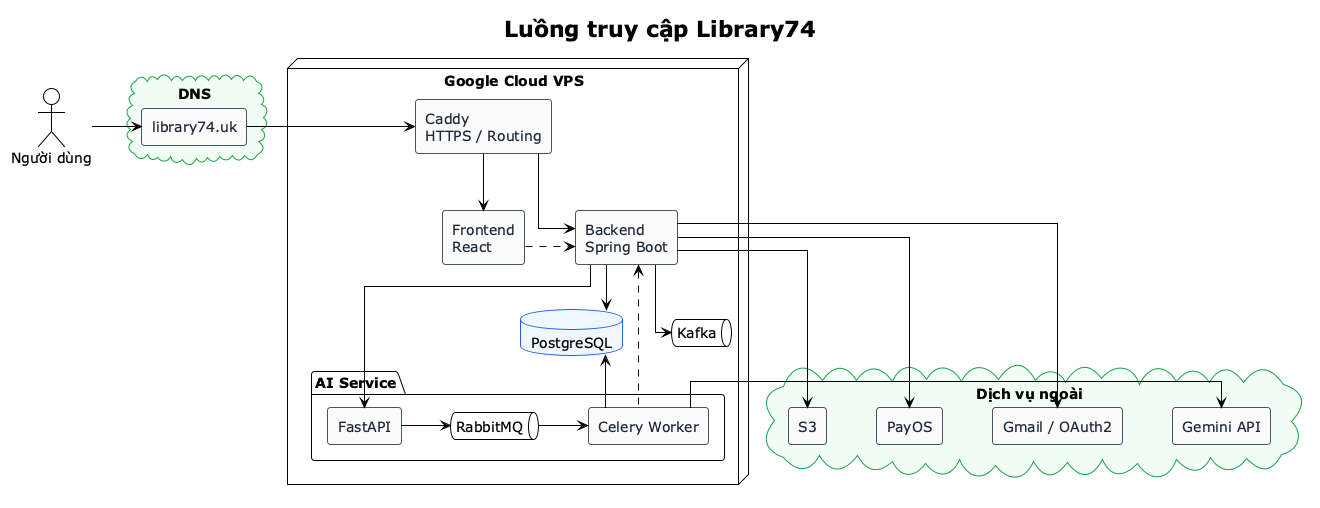
\includegraphics[width=0.95\textwidth]{figures/ch09/dns_flow.png}
    \caption{Luồng kết nối từ tên miền Library74 đến hệ thống production}
    \label{fig:dns_flow}
\end{figure}

\subsection{Tổng chi phí vận hành}

Bảng~\ref{tab:hosting_cost} được điều chỉnh theo chi phí triển khai hiện tại.
Tên miền \texttt{library74.uk} được mua theo năm, còn máy chủ demo đang chạy
trên Google Cloud Platform với cấu hình ước tính khoảng 92 USD/năm. Tại thời
điểm triển khai demo, GCP đang có ưu đãi miễn phí 3 tháng nên chi phí thực trả
ban đầu thấp hơn chi phí vận hành ổn định về sau.

\begin{table}[h]
\centering
\small
\caption{Chi phí vận hành hệ thống trong cấu hình demo}
\label{tab:hosting_cost}
\begin{tabularx}{\textwidth}{|p{3.5cm}|p{3.3cm}|p{2cm}|X|}
\hline
\textbf{Thành phần} & \textbf{Chi phí} & \textbf{Chu kỳ} & \textbf{Ghi chú} \\
\hline
Tên miền \texttt{library74.uk} & 5,3 USD & Năm & Khoản bắt buộc để giữ địa chỉ public của demo. \\
\hline
SSL/HTTPS & Miễn phí & 90 ngày hoặc tự động & Let's Encrypt hoặc chứng chỉ tự động từ reverse proxy/nhà cung cấp. \\
\hline
Google Cloud Platform & 92 USD & Năm & Chi phí theo cấu hình máy chủ demo; hiện đang được miễn phí 3 tháng đầu. \\
\hline
Lưu trữ file & Theo mức sử dụng & Tháng & Ảnh bìa/PDF dùng object storage hoặc cấu hình tương đương; chi phí phụ thuộc dung lượng thực tế. \\
\hline
API ngoài & Miễn phí trong phạm vi demo & Tháng & Google OAuth, Gmail SMTP, PayOS sandbox/quota demo và Gemini quota thử nghiệm. \\
\hline
\textbf{Tổng cố định ước tính} & \textbf{97,3 USD} & \textbf{Năm} & Chưa tính ưu đãi miễn phí 3 tháng GCP và chi phí phát sinh theo dung lượng/request thực tế. \\
\hline
\end{tabularx}
\end{table}

\noindent Như vậy, sau giai đoạn miễn phí ban đầu, chi phí cố định tối thiểu của
hệ thống chủ yếu gồm tên miền và máy chủ GCP, khoảng 97,3 USD/năm theo cấu hình
demo. Khi triển khai production thật, nhóm cần cập nhật lại theo dung lượng PDF,
số lượt truy vấn AI và chính sách giá của nhà cung cấp tại thời điểm vận hành.
